\section{Testy}

W poniższym rozdziale przedstawione zostaną testy systemu. Zostały one wykonane na różnych etapach prac. Część widoków została utworzona specjalnie do tego, aby przetestować różne funkcjonalności systemu, a nie znajdą się w finalnej wersji produktu.

\newline \newline
Do pierwszych testów tworzenia zrzutów ekranu oraz pobierania listy aktywnych procesów napisano aplikację Windows Form, która po kliknięciu na przycisk "Zrzut" wyświetlany jest zrzut ekranu oraz lista procesów.

\begin{figure} [!ht]
    \centering
    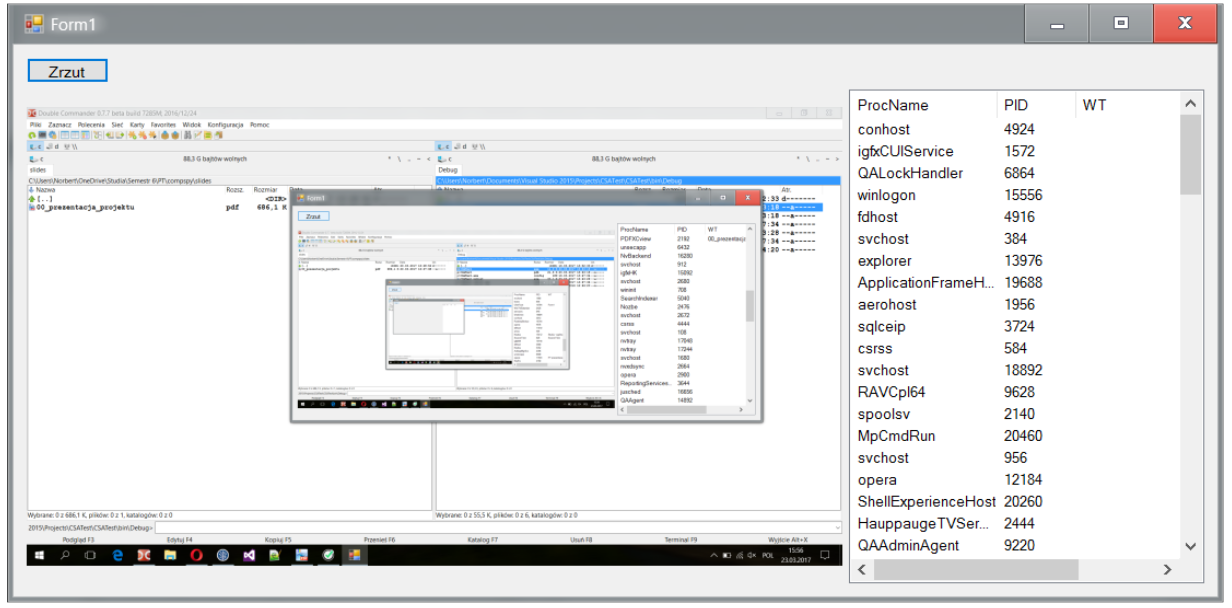
\includegraphics[height=9cm,width=16cm]{comspy_testy1}
    \caption{Testowanie funkcjonalności tworzenia zrzutów ekranu oraz pobierania listy aktywnych procesów.}
    \label{fig:my_label}
\end{figure}

\newpage
Gdy już udało się wybrać odpowiednie rozwiązanie postanowiono zbudować okno do podglądu w aplikacji klienta, aby można było sprawdzić działanie jeszcze przed połączeniem się do serwera i wysłaniem komunikatu. W tej wersji (w porównaniu do poprzedniego programu) działa również podgląd adresów i tytułów otwartych kart w przeglądarkach, a także zmiana jakości obrazu (niska i wysoka jakość). We wcześniejszej wersji korzystano także z funkcjonalności zegara do aktualizacji co określony czas.


\begin{figure} [!ht]
    \centering
    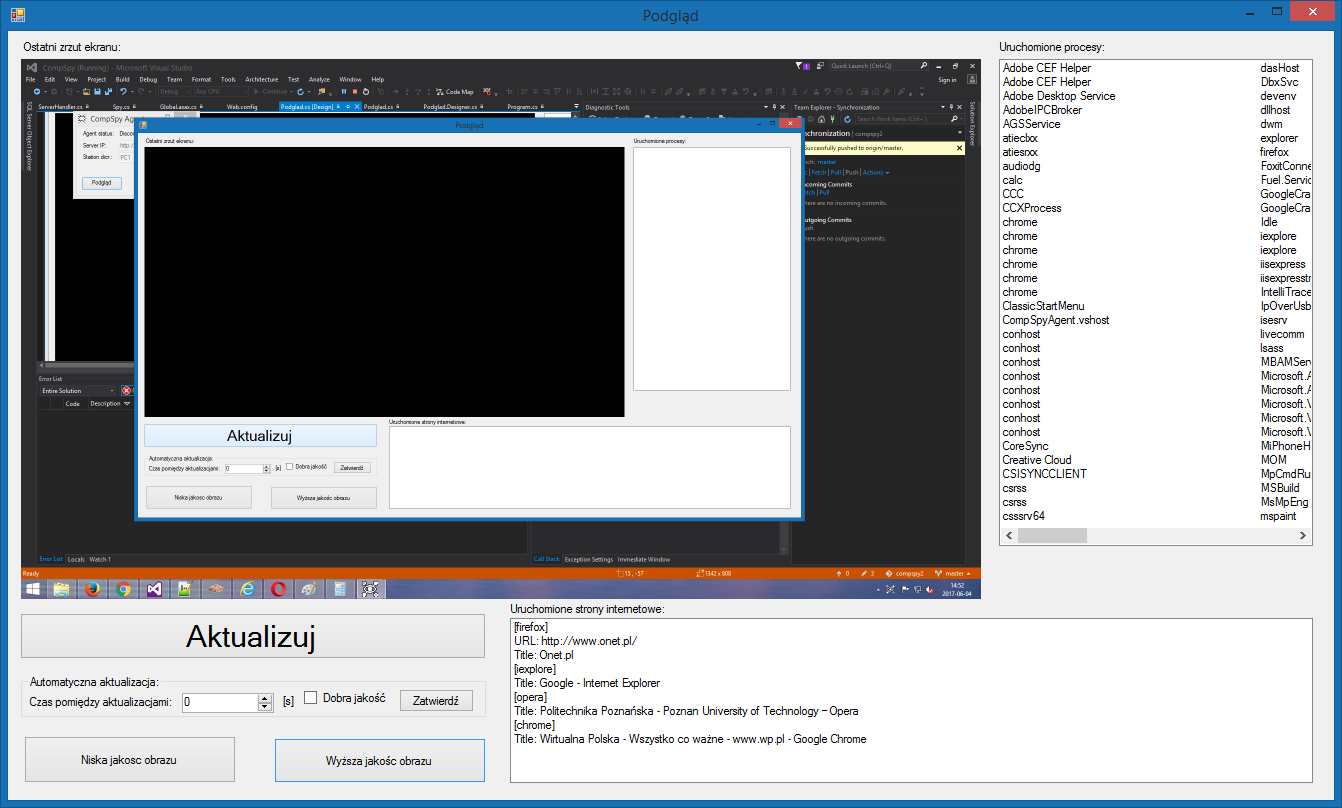
\includegraphics[height=9cm,width=16cm]{comspy_testy3}
    \caption{Widok Podgląd w aplikacji klienta}
    \label{fig:my_label}
\end{figure}

\newpage
Gdy udało się połączyć aplikację klienta i serwer z pomocą biblioteki SignalR zaczęto także testować uruchamianie z poziomu strony metod wywoływanych u klienta. Rysunek nr 17 przedstawia możliwe przykładowe wykorzystanie takiego połączenia.

\begin{figure} [!ht]
    \centering
    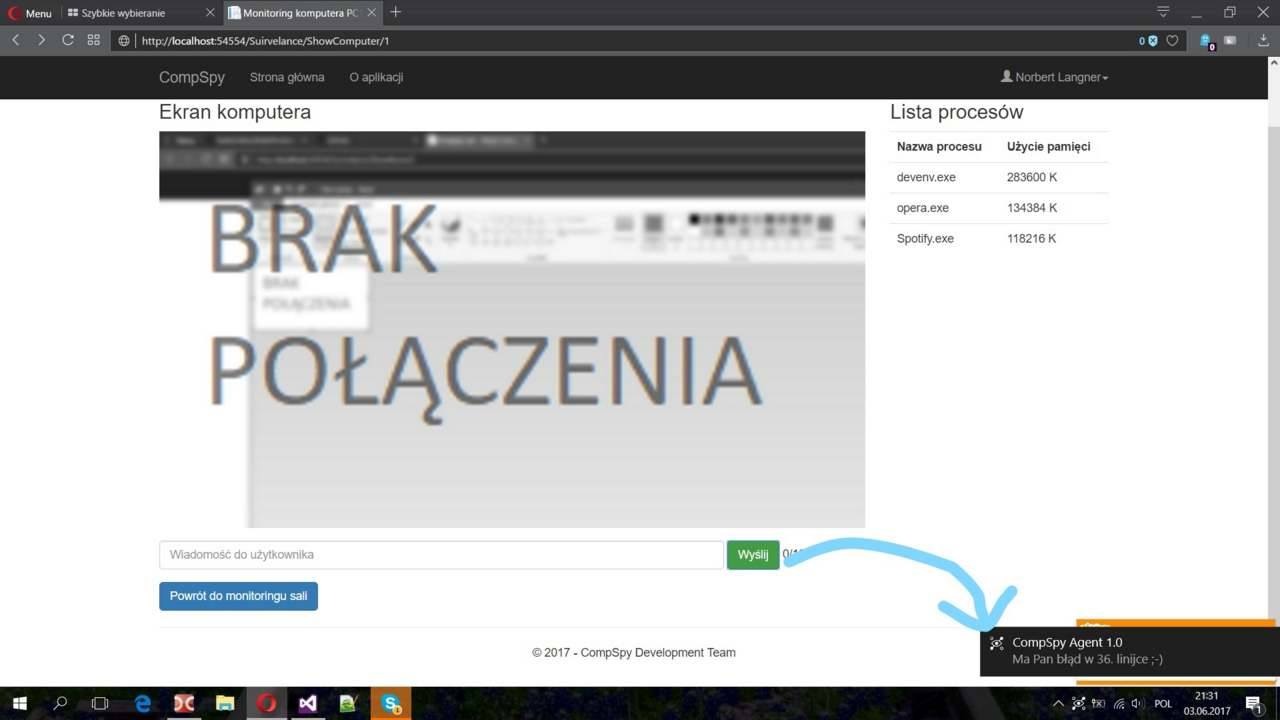
\includegraphics[height=9cm,width=16cm]{comspy_testy4}
    \caption{Testowanie funkcjonalności SignalR za pomocą wysyłania wiadomości do aplikacji klienta.}
    \label{fig:my_label}
\end{figure}

\newpage
Ostatni przedstawiony test miał już miejsce po wysłaniu poprawnego komunikatu przez klienta do serwera. Za pomocą narzędzi deweloperskich dostępnych w przeglądarce Opera sprawdzono otrzymany komunikat.

\begin{figure} [!ht]
    \centering
    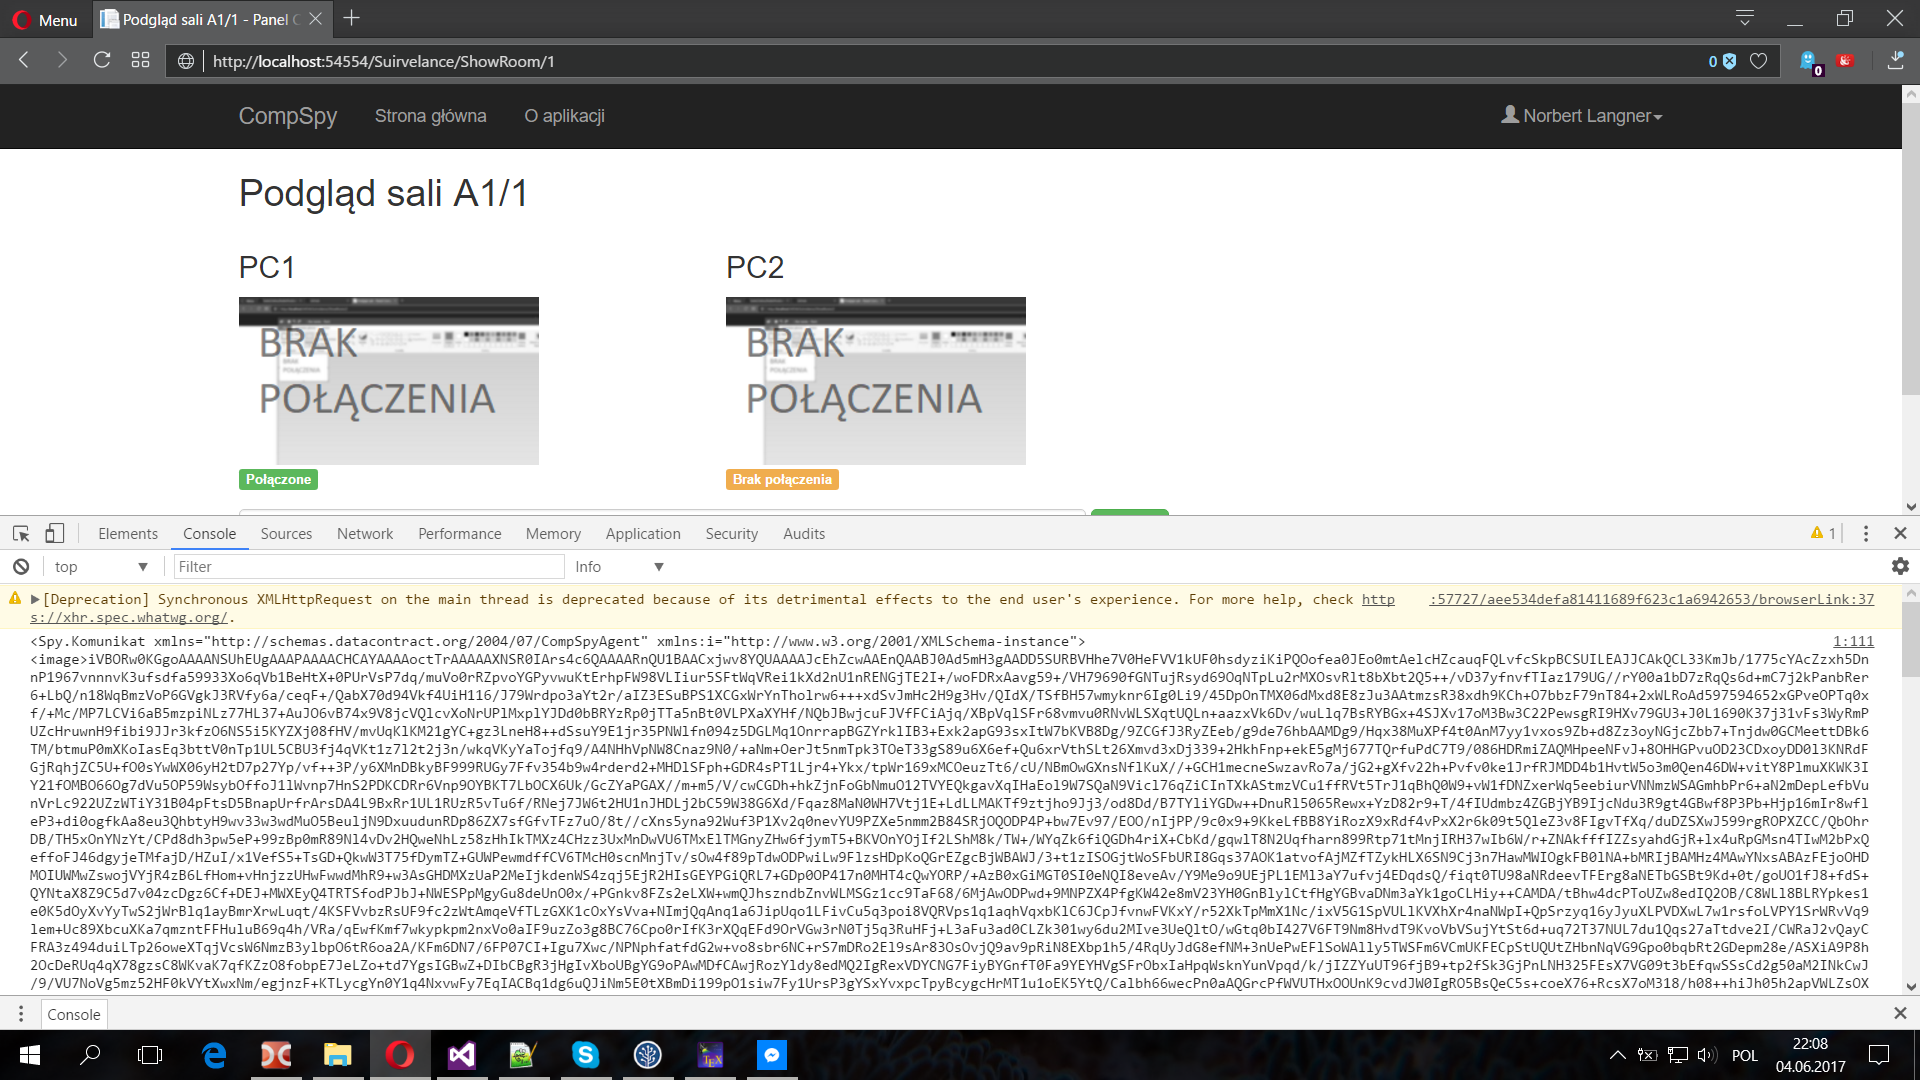
\includegraphics[height=9cm,width=16cm]{comspy_testy9}
    \caption{Podgląd komunikatu otrzymanego od klienta}
    \label{fig:my_label}
\end{figure}